\chapter{実装}
\label{implementation}

本章では,~\ref{method:approach}節で述べた手法を用いて純正のHoneypotにどのようなコマンドを実装し,Honeypot特有の異常な挙動を修正したのかを説明する.

\section{実装環境}
\label{implementation:env}
TBD
%本研究で実装するシステムを構成するためのハードウェアおよびソフトウェアについて説明する.表\ref{table:usedversion}に詳細なバージョンを示す.

%\begin{table}[!hbtp]
%    \begin{center}
%        \caption{使用ソフトウェアおよびハードウェアのバージョン}
 %       \begin{tabular}{|c|c|c|}
 %           \hline
 %           ハードウェア/ソフトウェア & 実装環境 & バージョン\\
%            \hline
%            \hline
%            シングルボードコンピュータ & Raspberry Pi3 & ModelB \\
%            \hline
%            3Dプリンタ & simple metal & 1403 \\
%            \hline
%            3Dプリンタ制御 & Octoprint & 1.3.0 \\
%            \hline
%            Blockchainクライアント & Geth & 1.5.8 \\
%            \hline
%            アプリケーションフレームワーク & laravel & 5.2 \\
%            \hline
%        \end{tabular}
%        \label{table:usedversion}
%    \end{center}
%\end{table}

%\subsection{ハードウェア}
%\label{implementation:hardware}
%3Dプリンタを制御およびBlockchainへの製造情報の保存を行うためのシングルボードコンピュータとしてRaspberry Pi3を用いる\cite{RaspberryPi}.Raspberry Pi3は安価に購入でき,LinuxベースのOSによって動作する.そのため,Blockchainノードとして正常に動作せることが可能である.また,USBポートで3Dプリンタを接続し,制御するソフトウェアもいくつか存在する.


%今回の実装では,3Dプリンタとしてprintrbot社のsimple metalを用いる\cite{Printrbot}.simple metalはSLA法の個人向け3Dプリンタであり,比較的安価なモデルである.USBポートによってコンピュータを接続することで制御を行うことができる.

%\subsection{3Dプリンタの制御}
%\label{implementation:ctl3dprinter}

%本システムでは,3Dプリンタを制御するシステムとして,Octoprint\cite{octoprint}を用いる.Octoprintはオープンソースの3Dプリンタ制御ソフトウェアであり,Raspberry Piに導入し,Webインターフェースよりプリントを行うことができる.3Dモデルの形式は一般的なSTL形式ではなく,3Dプリントを実際に行う際の制御コマンド体系であるG-CODE形式で入力を行う.多くの機能がRESTfulなAPIで実装されており,3Dプリンタを制御しながら他のアプリケーションへ容易に連携させることが可能である.

%\subsection{Blockchainへのデータ保存}
%\label{implementation:savedata}

%本システムでは,Blockchainに製造情報を保存する方法として,\ebc{}のCAとして保存する.EthereumはBlockchainを用いたアプリケーション開発プラットフォームとしては最も一般的に使われている.そのため本システムで独自にBlockchainを構築し十分にスケールさせなくとも,Blockchainの高改ざん耐性を利用することができる.また,Ethereum上で動作するプログラムはチューリング完全性を持つため,データ構造などを比較的自由に記述することができる.Ethereumのクライアントとしては,Go言語で実装されたGeth\cite{geth}を用いる.GethはJSON-RPCによるAPIが実装されており,プログラムから制御できる.

%\subsection{システム全体}
%\label{implementation:system}
%本システムは,本節で述べた複数のソフトウェアを連携させて動作する.今回は,全体をコントロールするインターフェイスとしてWebブラウザからアクセスすることを想定した.そこで,PHPによるWebアプリケーションフレームワークであるLaravel\cite{laravel}を用いて実装した.Laravelは2012年にリリースされてから急速に普及しているPHPフレームワークであり,オープンソース化されている.

%\section{データ登録システム}

%ユーザが3Dプリントを行う際のシーケンス図を以下に示す.ユーザが3Dプリントを命令した際にJSON RPCよりEthereum上にコントラクトをデプロイし,そのCAのアドレスをプリントされる製造物のIDとする.このIDを製造物の内部にRFIDを埋め込むなどで製造物と紐付け,製造物からコントラクトを呼び出すことができ,追跡可能性を担保する.デプロイされたコントラクトはマイナーによって実際にブロックへ格納され,後日改ざんすることは困難になる.

%\begin{figure}[h]
%    \begin{center}
%        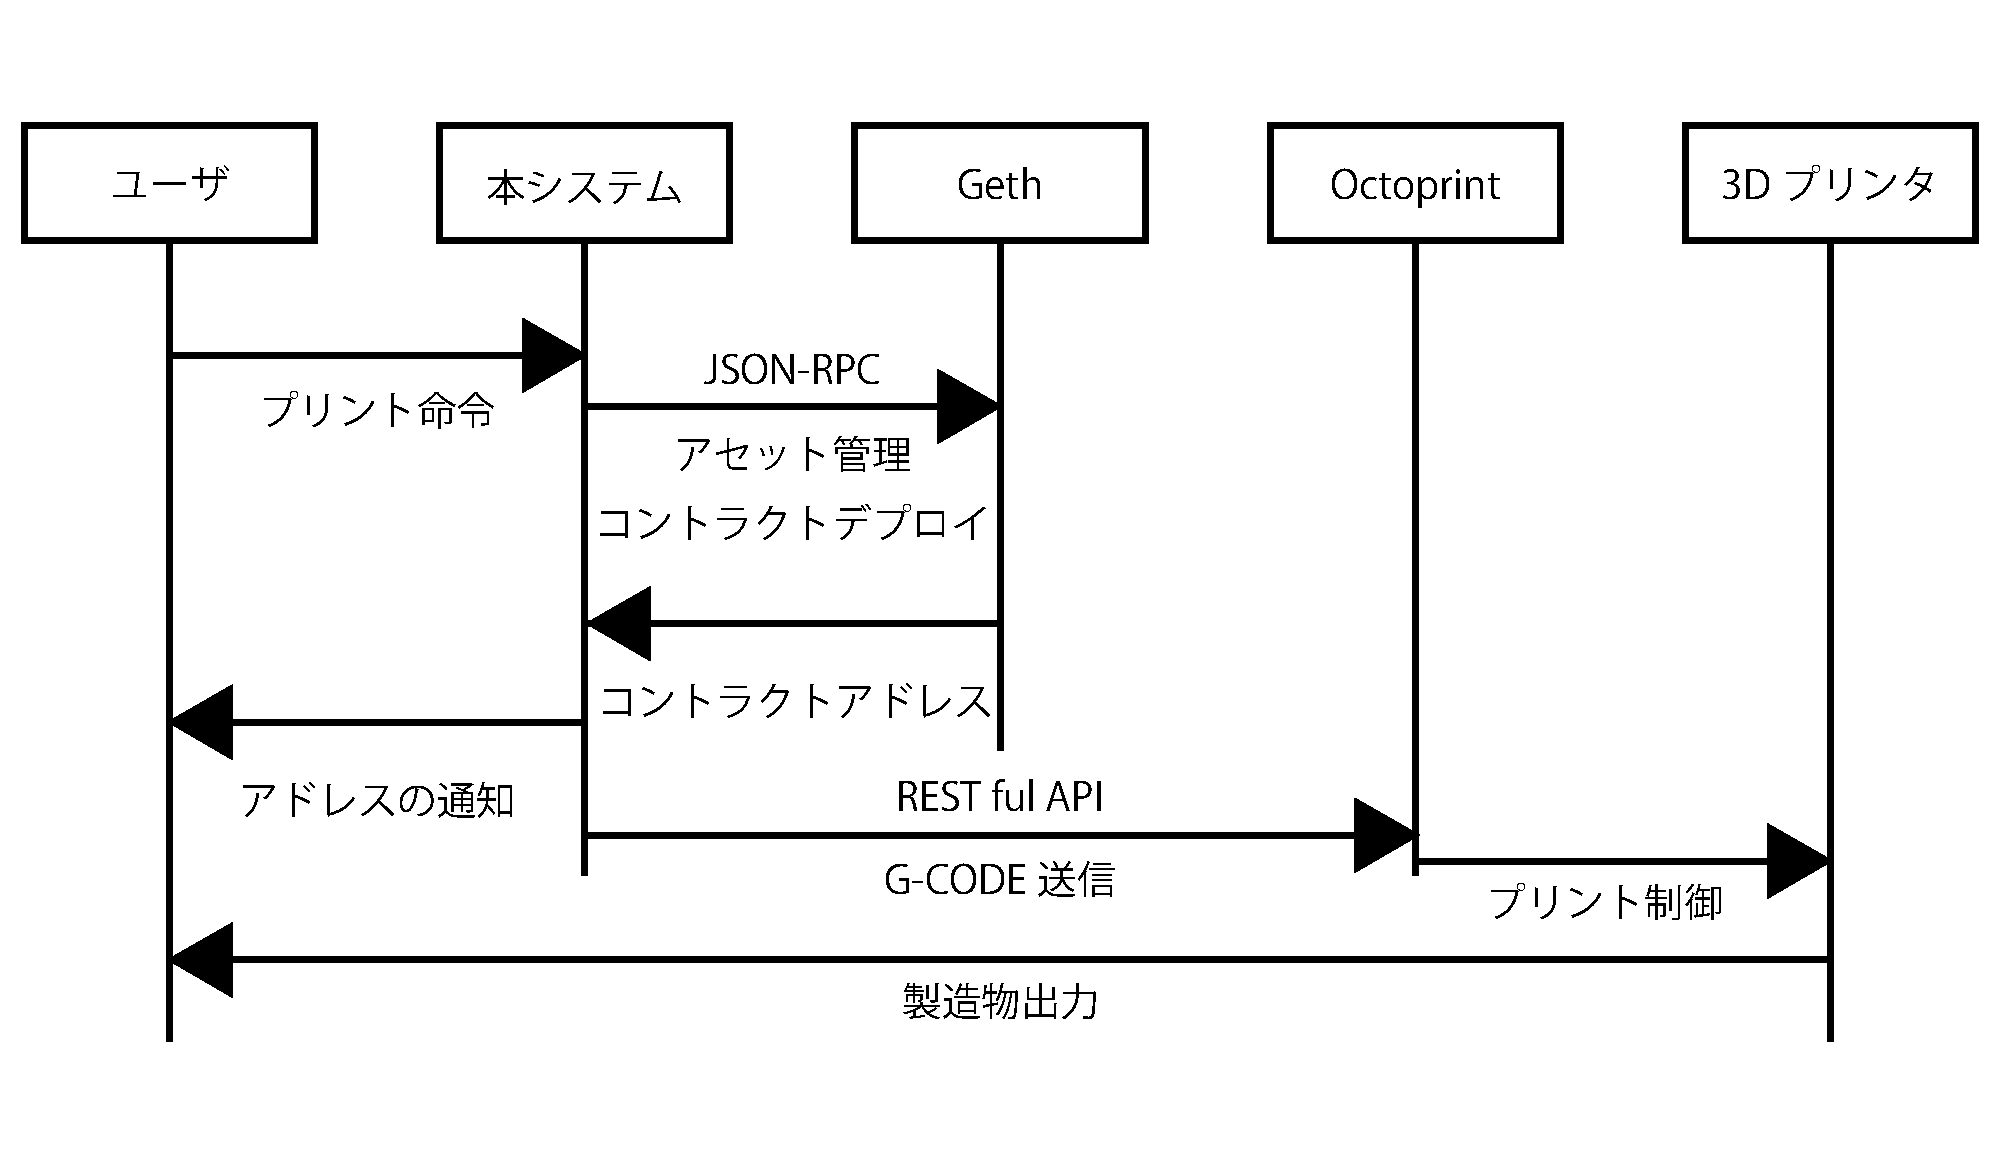
\includegraphics[scale=0.4]{./img/si-kensu.pdf}
%        \caption{システムシーケンス図}
%        \label{img:sequence}
%    \end{center}
%\end{figure}

%\subsection{保存するデータ構造}
%製造物の製造責任の追及,および知的財産権の保証には,製造物の設計図となる3Dモデル,3Dモデルの設計者,製造者,製造日時の記録が必要である.3Dモデルの設計者の担保を行うためには3Dモデルにデジタル署名が埋め込まれている必要があるが,現状では埋め込まれていない.また,製造日時については,P2Pネットワークにおいて特定のノードが述べる日時が正しいことを保証することはできないため,製造時に保存したとしても信頼出来るデータとは限らない.そこで本実装では3Dモデル,製造物の名前,製造者のみを保存する.Ethereumでは3Dモデルを直接Blockchainに保存することはEthereum上に保存できるデータ容量の制限により不可能なため,3Dモデルのハッシュ値を保存する.ハッシュ値を参照することで,製造物をプリントした3Dモデルと同様のデータであることを検証可能とする.また,製造者のデータとしてはEthereumのアドレスを使う.

%\begin{table}[!hbtp]
%    \begin{center}
%        \caption{保存するデータ構造}
%        \begin{tabular}{|c|c|c|}
%            \hline
%            Label & データサイズ &  概要\\
%            \hline
%            \hline
%            name & 最大32byte & 製造物の名前 \\
%            \hline
%            3d data hash & 32byte & SHA256を用いた3Dモデルのハッシュ値 \\
%            \hline
%            maker & 32byte  & 製造者のEthereumアドレス \\
%            \hline
%        \end{tabular}
%        \label{table:dataconstracture}
%    \end{center}
%\end{table}

\subsection{純正のHoneypotで未実装のコマンドの実装}
\label{implementation:ImplBusyBox}
本研究において純正のHoneypotはCowrie\cite{cowrie}を使用し,実際のShellには実装されているが,純正のHoneypotで未実装のコマンドについてはBusyBox\cite{busybox}に含まれるコマンドの実装を行なった.2.1.1.2や2.2.2で紹介した通り,BusyBoxに含まれるコマンドの種類が219ある中で,Cowrieの実装コマンド数は38しか存在しない.この差分をPythonで実装する.\\
実装例は以下の通り.(付録にて例で紹介できなかったコマンドを掲載する)\\


%%% Local Variables:
%%% mode: japanese-latex
%%% TeX-master: "../bthesis"
%%% End:
